\chapter{Impacto Medioambiental}
\label{cap:ImpactoMedioAmbiente}

En 2015, la ONU aprobó la \emph{Agenda 2030 sobre el Desarrollo Sostenible}\cite{agenda2030}, una oportunidad para que los países y sus sociedades evolucionen y mejoren la vida de todos, sin dejar a nadie atrás. Constituye un llamamiento universal a la acción para poner fin a la pobreza, proteger el planeta y mejorar la vida de personas y animales. Se aprobaron entonces 17 objetivos\cite{17objetivos} a alcanzar en 15 años. \\

Dentro de los 17 objetivos, hay 2 muy importantes en los que la aplicación Estublock tiene un impacto negativo en el presente pero este se minimizará muy pronto. La tecnología blockchain aporta sin duda una gran cantidad de ventajas, como la fiabilidad, transparencia de las operaciones (el código de los smart contracts esta a disposición de la gente), seguridad de los datos, inmutabilidad, anonimato\dots Pero, una de estas ventajas trae consigo una desventaja a nivel medioambiental. Como sabemos, una red blockchain es \emph{descentralizada}, esto se debe a que hay varios nodos conectados entre si. Cada nodo es un ordenador en ejecución, lo que implica que cada ordenador esta las veinticuatro horas del día encendido, los siete días de la semana y los 12 meses del año. Esto multiplicado por cada ordenador que hay en la red blockchain. Por ejemplo, la red de bitcoin dispone a día de hoy \textit{2021-05-24} de 9786 nodos\cite{bitcoinNodos}. Pero no son solo nodos encendidos, sino que un punto muy importante es el algoritmo de consenso que utiliza la red blockchain. En el caso de bitcoin y Ethereum versión 1, el algoritmo de consenso es \emph{Proof of Work} lo que hace que los nodos de la red estén constantemente ``minando'' para encontrar el hash del próximo bloque. Este poder de computo requiere de mucha energía eléctrica, venga de fuentes sostenibles o no. \\

\begin{figure}[h!]
  \centering
  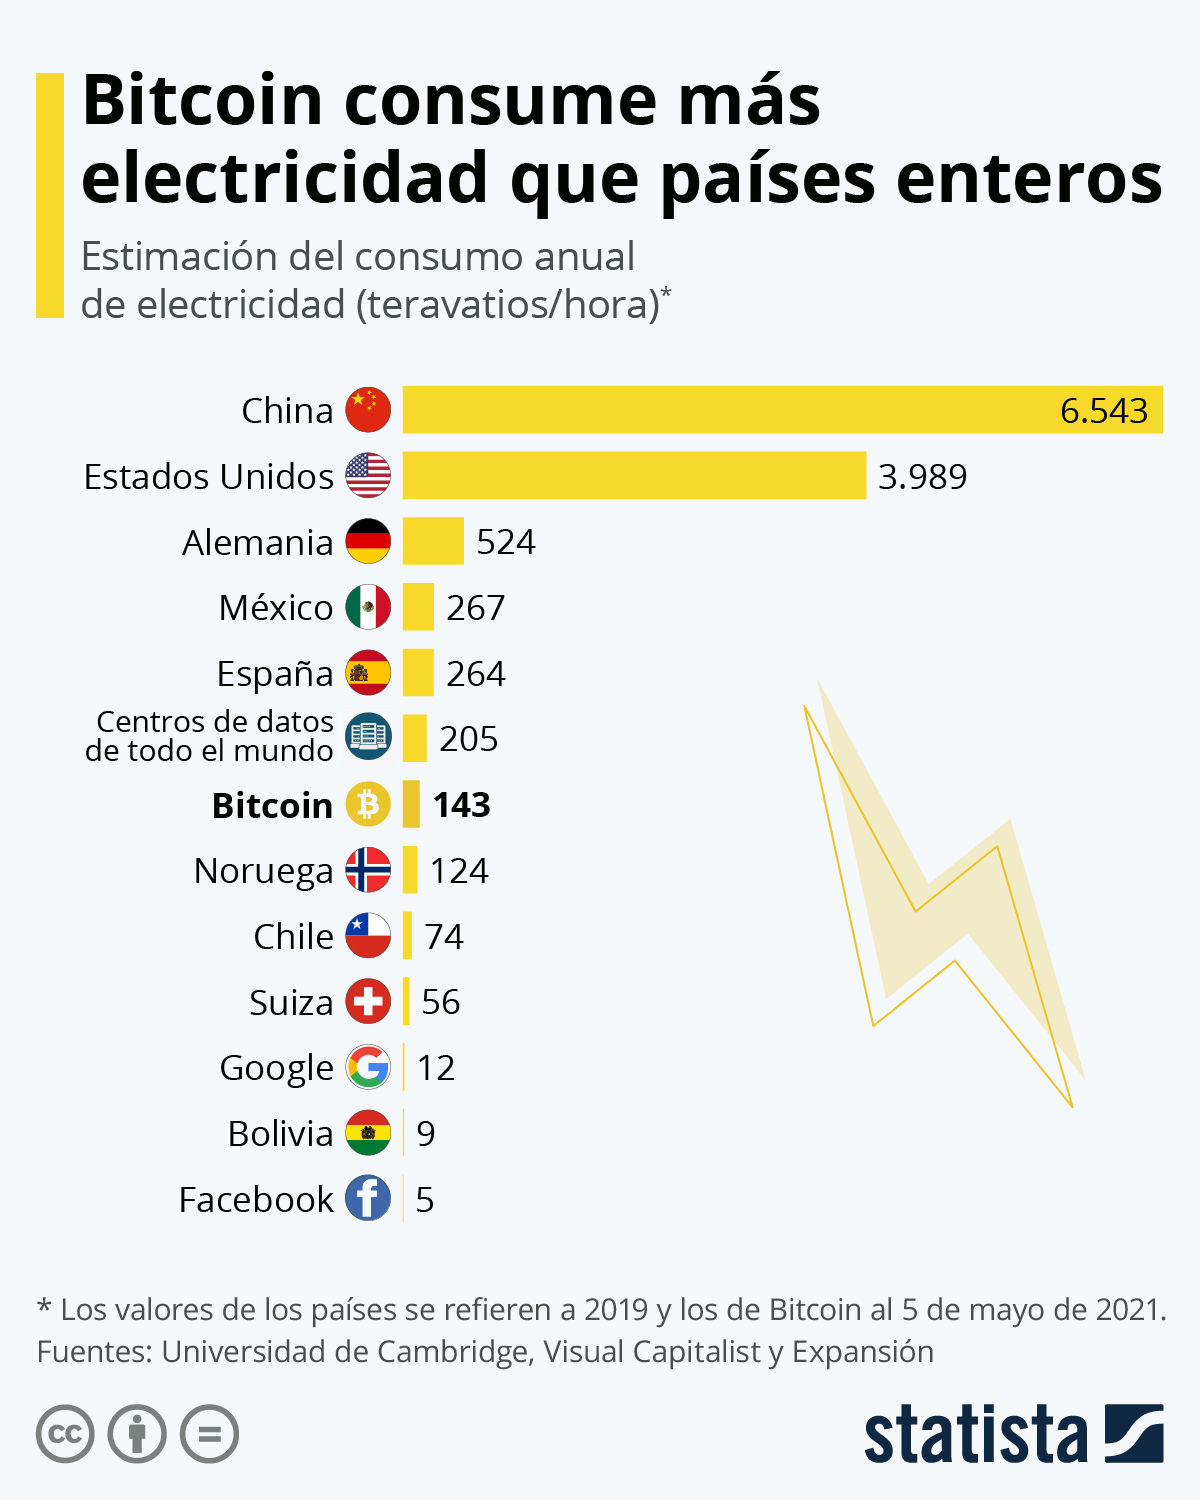
\includegraphics[width=0.4\linewidth]{figs/ImpactoMedioAmbiente/electricidad_bitcoin}
  \caption[Arquitectura]{Arquitectura Completa del proyecto}
  \label{fig:estublockArch}
\end{figure}

\clearpage
Por suerte, aunque parezca que blockchain va a consumir tanta energía como el \textit{Centro de Datos de Todo el Mundo}, en 2019 \emph{Coinshares} realizó una investigación\cite{coinshare} que reveló que el 74\% de las operaciones mineras se realizan con energía renovable. Sin embargo, siempre se puede mejorar, y llegar al 100\% y además, se puede minimizar al máximo el consumo de energía. Y es aquí donde entra \emph{Ethereum versión 2}\cite{Ethereum2.0}. Al cambiar el algoritmo de consenso de \textit{Proof of Work} a \textit{Proof of Stake}, ethereum disminuirá enormemente el consumo de energía. Hasta tal punto, de que \textbf{Joseph Pallant}, fundador de la \emph{blockchain for climate foundation}\cite{bkClimateF} utiliza Ethereum2.0. Aunque esta segunda versión de Ethereum ya esta en funcionamiento, se requiere de un tiempo para migrar los datos de la versión 1 a la 2, pero con el tiempo la versión 2 de ethereum crecerá, disminuyendo enormemente el gasto energético que conlleva. \\

Así pues, Estublock utiliza actualmente la red de Ethereum con un gasto energético casi nulo, pero hay que tener en cuenta que aunque la red gaste poco, hay varios ordenadores encendidos consumiendo energía. Uno de los objetivos de desarrollo sostenible es el \textbf{9} ``Industria, Innovación e Infraestructura'', Estublock requiere de varios nodos en la red blockchain para funcionar, y para que tenga sentido utilizar una red blockchain. Creo que el gasto energético es muy bajo, pero no se nos puede olvidar que gastar energía, gasta y que sería recomendable lograr que los ordenadores estén lo más especializados posible para minimizar al máximo el gasto energético cumpliendo con el objetivo \textit{9.4} ``modernizar la infraestructura para que sean sostenibles''. También tiene un impacto en el punto \textbf{13} ``Acción por el Clima'' con respecto al objetivo de minimizar las emisiones de carbono al máximo, en las universidades en las que se utilice la aplicación Estublock y dispongan de nodos en la red blockchain, se puede tratar de utilizar siempre energías renovables como poner paneles solares en la universidad para que los nodos de la red utilicen esa energía renovable para funcionar.

